\subsection{Scheduling}\label{subsec:Scheduling}
CPU scheduling is the basis of multiprogrammed operating systems.
In a single-processor system, only one process can run at a time.
Others must wait until the CPU is free and can be rescheduled.
By switching the CPU among processes, the operating system can maximize CPU utilization.

For example, a \nameref{def:Process} is executed until it must wait.
Typically the process waits for the completion of some I/O request.
In a simple computer system, the CPU then just sits idle.
All this waiting time is wasted; no useful work is accomplished.

\begin{blackbox}
  \textbf{On operating systems that support them, \nameref{def:Kernel_Thread}s, not \nameref{def:Process}es are scheduled by the operating system.}
  However, the terms ``process scheduling'' and ``thread scheduling'' are often used interchangeably.
  Process scheduling is used when discussing general scheduling concepts and thread scheduling to refer to thread-specific ideas.
\end{blackbox}

Scheduling of this kind is a fundamental operating-system function.
Almost all computer resources are scheduled before use.

\subsubsection{CPU and I/O Bursts}\label{subsubsec:CPU_IO_Bursts}
To properly schedule a \nameref{def:Process}, its \nameref{def:CPU_Burst}s and \nameref{def:I/O_Burst}s need to observed.

\begin{definition}[CPU Burst]\label{def:CPU_Burst}
  A \emph{CPU burst} is one of the states of execution for a \nameref{def:Process}.
  This is the state when the process is actively using the CPU to perform computations.
  In this state, the CPU is performing activity for \textbf{this} \nameref{def:Process}, and \textbf{IS NOT} waiting for an I/O device to perform some action or return information.
\end{definition}

\begin{definition}[I/O Burst]\label{def:I/O_Burst}
  An \emph{I/O burst} is one of the states of execution for a \nameref{def:Process}.
  This is the state when the process is waiting on the I/O device to return the requested information or perform the desired action.
  In this state, the CPU is doing no activity for \textbf{this} \nameref{def:Process}.
\end{definition}

A \nameref{def:Process} alternates between these two bursts, with the final \nameref{def:CPU_Burst} terminating this \nameref{def:Process}'s execution.
The distribution of length of CPU bursts is an exponential or hyperexponential graph.
This means:
\begin{itemize}[noitemsep]
\item There is a large number of short duration CPU bursts.
\item There is a small number of long duration CPU bursts.
\end{itemize}

We can categorize these into either \nameref{def:CPU_Bound} programs or \nameref{def:IO_Bound} programs.
\begin{itemize}[noitemsep]
\item I/O-bound programs have a small number of CPU bursts which have a relatively short duration relative to the I/O operations.
  The I/O operations take up a majority of the time the \nameref{def:Process} executes.
\item CPU-bound programs have a large number of CPU bursts, which have a relatively long duration relative to the I/O operations.
  The CPU operatiosn take up a majority of the time the \nameref{def:Process} executes.
\end{itemize}

\subsubsection{CPU Scheduler}\label{subsubsec:CPU_Scheduler}
Whenever the CPU becomes idle, i.e.\ it has finished the current CPU burst early, or there is an I/O operation, the \nameref{def:Operating_System} must select the next \nameref{def:Process} and/or \nameref{def:Thread} to schedule.
This is handled by the \nameref{def:Short_Term_Scheduler}.

\begin{definition}[Short-Term Scheduler]\label{def:Short_Term_Scheduler}
  The \emph{short-term scheduler} is responsible for scheduling either the next \nameref{def:Process} or \nameref{def:Thread} for execution on the \textbf{CPU} from all the possible ones in memory.
  This is run quite frequently, every couple hundred milliseconds, usually.

  \begin{remark}[CPU Scheduler]\label{rmk:CPU_Scheduler}
    Because the \nameref{def:Short_Term_Scheduler} only schedules tasks for the CPU, it is also called the \emph{CPU Scheduler}.
  \end{remark}
\end{definition}

\paragraph{Preemption and Scheduling}\label{par:Preemption_Scheduling}
There are 4 times when CPU scheduling occurs:
\begin{enumerate}[noitemsep]
\item When a process switches from the \texttt{RUNNING} state to the \texttt{WAITING} state.
\item When a process switches from the \texttt{RUNNING} state to the \texttt{READY} state (for example, when an interrupt occurs).
\item When a process switches from the \texttt{WAITING} state to the \texttt{READY} state (for example, at completion of I/O).
\item When a process terminates.
\end{enumerate}

In the case of Times 1 and 4, there are no options in terms of scheduling.
In the first situation, a \nameref{def:Process} is being made unschedule-able by the \nameref{def:Operating_System}.
So, another process must be switched in for the one that was made to wait.
Similarly, when a \nameref{def:Process} terminates, there is no option for how to schedule it, because it's done executing.

A \nameref{def:Nonpreemptive_Kernel} only allows scheduling during Times 1 and 4.
In this system, once a \nameref{def:Process} gets allocated to the CPU, it keeps the CPU until it terminates, it switches to the \texttt{WAITING} state, or it voluntarily yields control of the CPU.

A \nameref{def:Preemptive_Kernel} allows scheduling during all Times (1--4).
This can only be done on certain hardware platforms (all major ones today), because a timer is needed, among other special hardware.
In this system, \nameref{def:Race_Condition}s appear.
We also need to design the \nameref{def:Kernel} to allow for \nameref{def:Preemption}, such as when the kernel is busy performing a \nameref{def:System_Call} for a \nameref{def:Process}.
If we don't have to worry about real-time computing, then we can wait for the \nameref{def:System_Call} to finish before moving onto another task.

\paragraph{Interrupt Handling}\label{par:Interrupt_Handling}
\nameref{def:Interrupt}s can happen \textbf{AT ANY TIME}, which must be accepted at almost all times.
On multiprocessor systems, it is costly to turn off interrupt handling on all cores, but sometimes it is necessary.
If we don't, input might be lost or output overwritten.
To ensure that these code sections are not accessed concurrently by several processes, they disable interrupts at entry and reenable interrupts at exit.
The sections of code that disable interrupts do not occur often and typically contain few instructions.

\paragraph{Dispatcher}\label{par:Dispatcher}
The \nameref{def:Dispatcher} \textbf{MUST} be as fast as possible to minimize the amount of time spent working on switching betweeen \nameref{def:Process}es/\nameref{def:Thread}s.
This is measured as the \nameref{def:Dispatch_Latency}.

\begin{definition}[Dispatcher]\label{def:Dispatcher}
  The \emph{dispatcher} is a \nameref{def:Short_Term_Scheduler} function.
  It is the code responsible for giving control of the CPU to the \nameref{def:Process} that the scheduler selected.
  This involves:
  \begin{enumerate}[noitemsep]
  \item Performing a \nameref{def:Context_Switch}.
  \item Switching to the appropriate mode, \nameref{def:User}-mode or \nameref{def:Kernel}-mode.
  \item Jumping to the proper location in the \nameref{def:Process} to continue its execution.
  \end{enumerate}
\end{definition}

\begin{definition}[Dipatch Latency]\label{def:Dispatch_Latency}
  The \emph{dispatch latency} is the amount of time required by the \nameref{def:Dispatcher} to stop one \nameref{def:Process} and switch to another.
\end{definition}

\subsubsection{Scheduling Criteria}\label{subsubsec:Scheduling_Criteria}
The choice of how to schedule tasks for the CPU is completely dependent on the desired outcome of the scheduling algorithm and the desired performance of the system.
The criteria for most algorithms are:
\begin{itemize}[noitemsep]
\item \textbf{CPU utilization}.
  We want to keep the CPU as busy as possible.
  In a real system, it utilization should range from 40 percent (for a lightly loaded system) to 90 percent (for a heavily loaded system).
\item \textbf{Throughput}.
  If the CPU is busy executing processes, then work is being done.
  The number of processes that are completed per time unit is called throughput.
\item \textbf{Turnaround time}.
  From the point of view of a process, the important criterion is how long it takes to execute that process.
  The interval from the time of submission of a process to the time of completion is the turnaround time.
  This includes time spent waiting to get into memory, waiting in the ready queue, executing on the CPU, and doing I/O.
\item \textbf{Waiting time}.
  The CPU-scheduling algorithm does not affect the amount of time during which a process executes or does I/O, only the amount of time that a process spends in the ready queue.
  Waiting time is the sum of the periods spent waiting in the ready queue.
\item \textbf{Response time}.
  In an interactive system, turnaround time may not be the best criterion.
  A process can produce some output early and then continue computing new results while previous results are being output to the user.
  Thus, another measure is the time from the submission of a request until its response is produced.
  This measure, called response time, is the time it takes to start responding, not the time it takes to output the response.
  The turnaround time is generally limited by the speed of the output device.
\end{itemize}

It is desirable to maximize CPU utilization and throughput and to minimize turnaround time, waiting time, and response time.
Usually the average measure is optimized.
However, sometimes it is better to optimize the minimum or maximum values rather than the average.

\subsubsection{Scheduling Algorithms}\label{subsubsec:Scheduling_Algorithms}
Here, we will discuss the different kinds of \nameref{def:Scheduling_Algorithm}s used by the \nameref{def:Short_Term_Scheduler}.

\begin{definition}[Scheduling Algorithm]\label{def:Scheduling_Algorithm}
  The \emph{scheduling algorithm} is responsible for choosing the next \nameref{def:Process}/\nameref{def:Thread} to run from the set of all \texttt{READY} processes.
\end{definition}

\paragraph{First-Come First-Served Scheduling}\label{par:FCFS_Scheduling}
In this algorithm, the first task that becomes \texttt{READY} is the first to execute.
This is easily handled with a FIFO queue.
The most recent task to appear in the task queue is appended as the tail of the FIFO queue's list, and moves forward until it gets to execute.
Once it has its chance to execute, this \nameref{def:Process} will execute for its entire period, making this a nonpreemptive scheduling method.

The problem with FCFS scheduling is the average waiting time for \nameref{def:Process}es, especially if there is a large difference in the amount of CPU time required by some of the processes.
This is illustrated visually in \Cref{fig:Gantt_Chart}.

\begin{example}[]{FCFS Calculations}
  Suppose 3 processes arrive at the same time and have these CPU bursts required.
  \begin{center}
    \begin{tabular}{cc}
      \toprule
      Process & Time Required \\
      \midrule
      $P_{1}$ & 24 \\
      $P_{2}$ & 3 \\
      $P_{3}$ & 3 \\
      \bottomrule
    \end{tabular}
  \end{center}
  \tcblower{}
  In a FCFS system, the average waiting time is
  \begin{equation*}
    \frac{0+24+27}{3} = \SI{17}{\milli \second}
  \end{equation*}

  However, if we were to schedule the short processes first, then the average waiting time would be
  \begin{equation*}
    \frac{0+3+6}{3} = \SI{3}{\milli \second}
  \end{equation*}
\end{example}

\begin{definition}[Gantt Chart]\label{def:Gantt_Chart}
  A \emph{Gantt chart} is a way to visualize the order and amount of time a processor spends executing a task.
  An example of one is shown in \Cref{fig:Gantt_Chart}.
  The start and end times of a particular task are also shown on the chart.
\end{definition}

\begin{figure}[h!tbp]
  \centering
  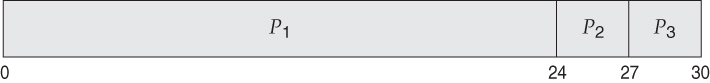
\includegraphics[scale=0.8]{./Drawings/EDAF35-Operating_Systems/Gantt_Chart.jpg}
  \caption{Gantt Chart}
  \label{fig:Gantt_Chart}
\end{figure}

Additionally, if there are a lot of small I/O tasks and just a few large CPU ones, then the \nameref{def:Convoy_Effect} starts.

\begin{definition}[Convoy Effect]\label{def:Convoy_Effect}
  The \emph{convoy effect} is a result of having few very CPU-intensive tasks that use the CPU fro their entire duration and a lot of small I/O-intensive tasks.
  There, the \nameref{def:CPU_Bound} task will block the \nameref{def:IO_Bound} tasks.
  This lowers overall throughput and device utilization.
\end{definition}

\paragraph{Shortest-Job-First Scheduling}\label{par:SJF_Scheduling}
Here, the job with the shortest amount of time required for the next CPU burst is scheduled first.
If 2 \nameref{def:Process}es have the same amount of time required, then the tie is broken with FCFS among those tasks.
This can be either preemptive or nonpreemptive.
The question comes up when a newly arrived \nameref{def:Process} has a shorter CPU burst than the one currently running.
If this new process preempts the currently running one, then it is a preemptive SJF scheduler, and is sometimes called \emph{Shortest-Remaining-Time-First scheduling}.

\begin{blackbox}
  Note that this is the length of the \textbf{next CPU burst}, not the overall length of CPU execution.
\end{blackbox}

%%% Local Variables:
%%% mode: latex
%%% TeX-master: "../../EDAF35-Operating_Systems-Reference_Sheet"
%%% End:
